\chapter{Badanie zachowania obiektu}
\label{sec:zad2}
Aby lepiej poznać naturę obiektu przeprowadzone zostały ogólne badania
zachowania obiektu i jego odpowiedzi na różne skoki wartości sterującej.
Eksperyment zakładał, iż na początku obiekt będzie w punkcie pracy
($Y = 3, U = 0,9$), a następnie, w chwili $k = 10$ wykonany zostanie skok
do zaplanowanej wcześniej wartości sterowania. Biorąc pod uwagę ograniczenia
na wartość sterowania $U^{min} = 0,6$ i $U^{max} = 1,2$ wartość sterowania
po skoku mieściła się w owym zakresie. Wyniki eksperymentu zostały zobrazowane
na wykresie \ref{fig:skoki}.
\begin{figure}
  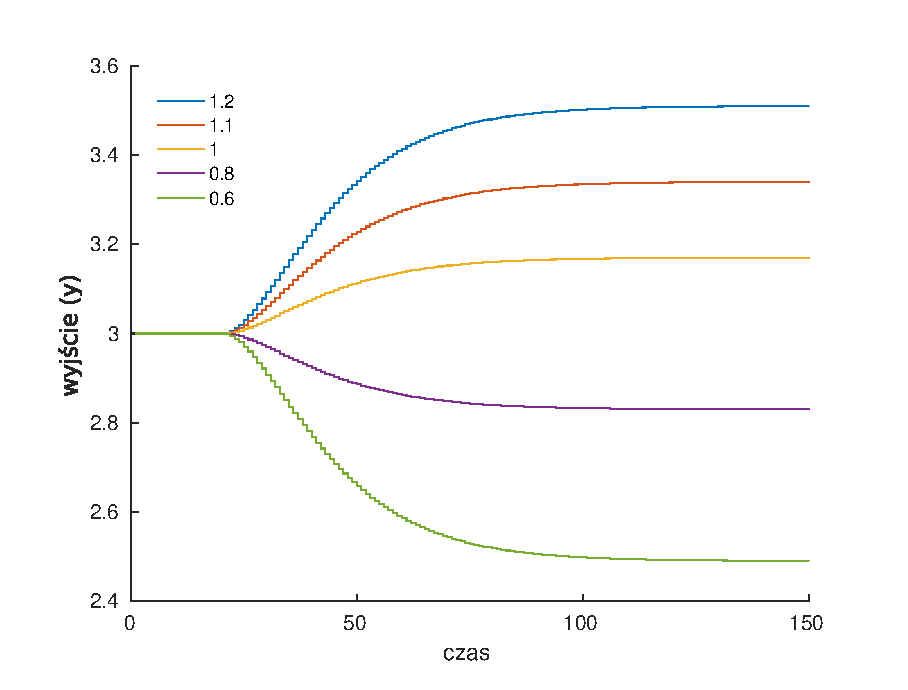
\includegraphics{wykresy/skoki.eps}
  \caption{Wyniki eksperymentu skoków do różnych wartości sterowania. Konkretne
  wartości zostały opisane w legendzie.}
  \label{fig:skoki}
\end{figure}
Następnie wyznaczona została charakterystyka statyczna obiektu. Znaleziona
została poprzez sprawdzenie przy jakiej wartości wyjścia obiekt stabilizuje
się dla danej wartości sterowania. Na podstawie tego sporządzony został wykres.
Wartości zostały zmierzone dla wartości pomiędzy ograniczeniam, z krokiem $0.01$.
Wyniki zostały zamieszczone na wykresie \ref{fig:char_stat}.
\begin{figure}
  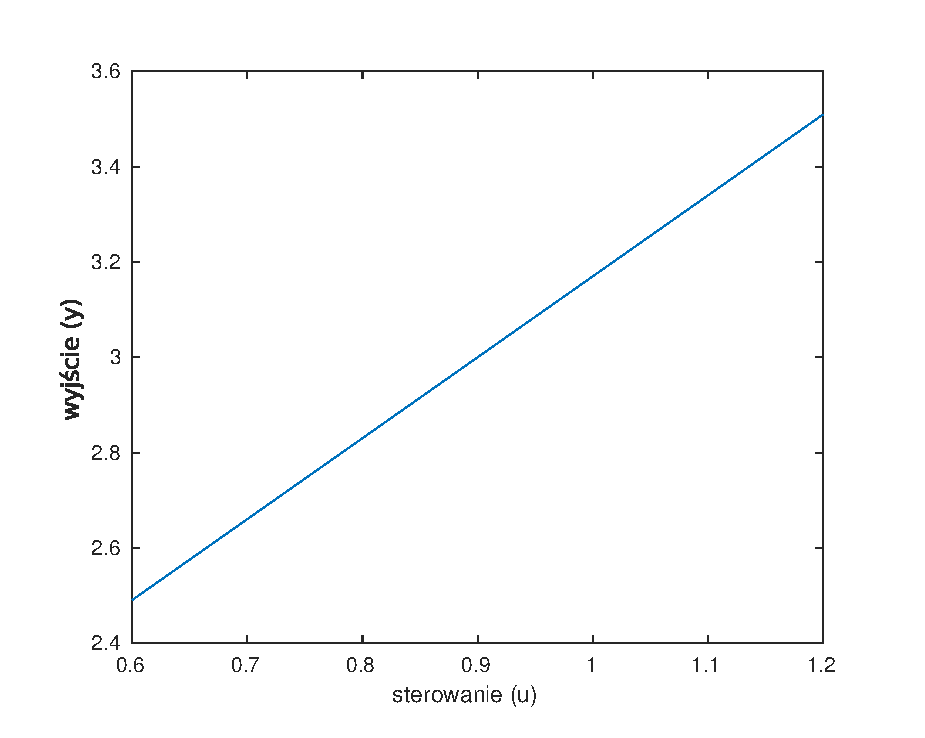
\includegraphics{wykresy/char_stat.eps}
  \caption{Charakterystyka statyczna obiektu.}
  \label{fig:char_stat}
\end{figure}
Otrzymana charakterystyka jest liniowa. Wzmocnienie statyczne, będące pochodną
charakterystyki statycznej ma wartość $1,7$.
